\documentclass{standalone}
\usepackage{tikz}
\usetikzlibrary{patterns, positioning}


\begin{document}
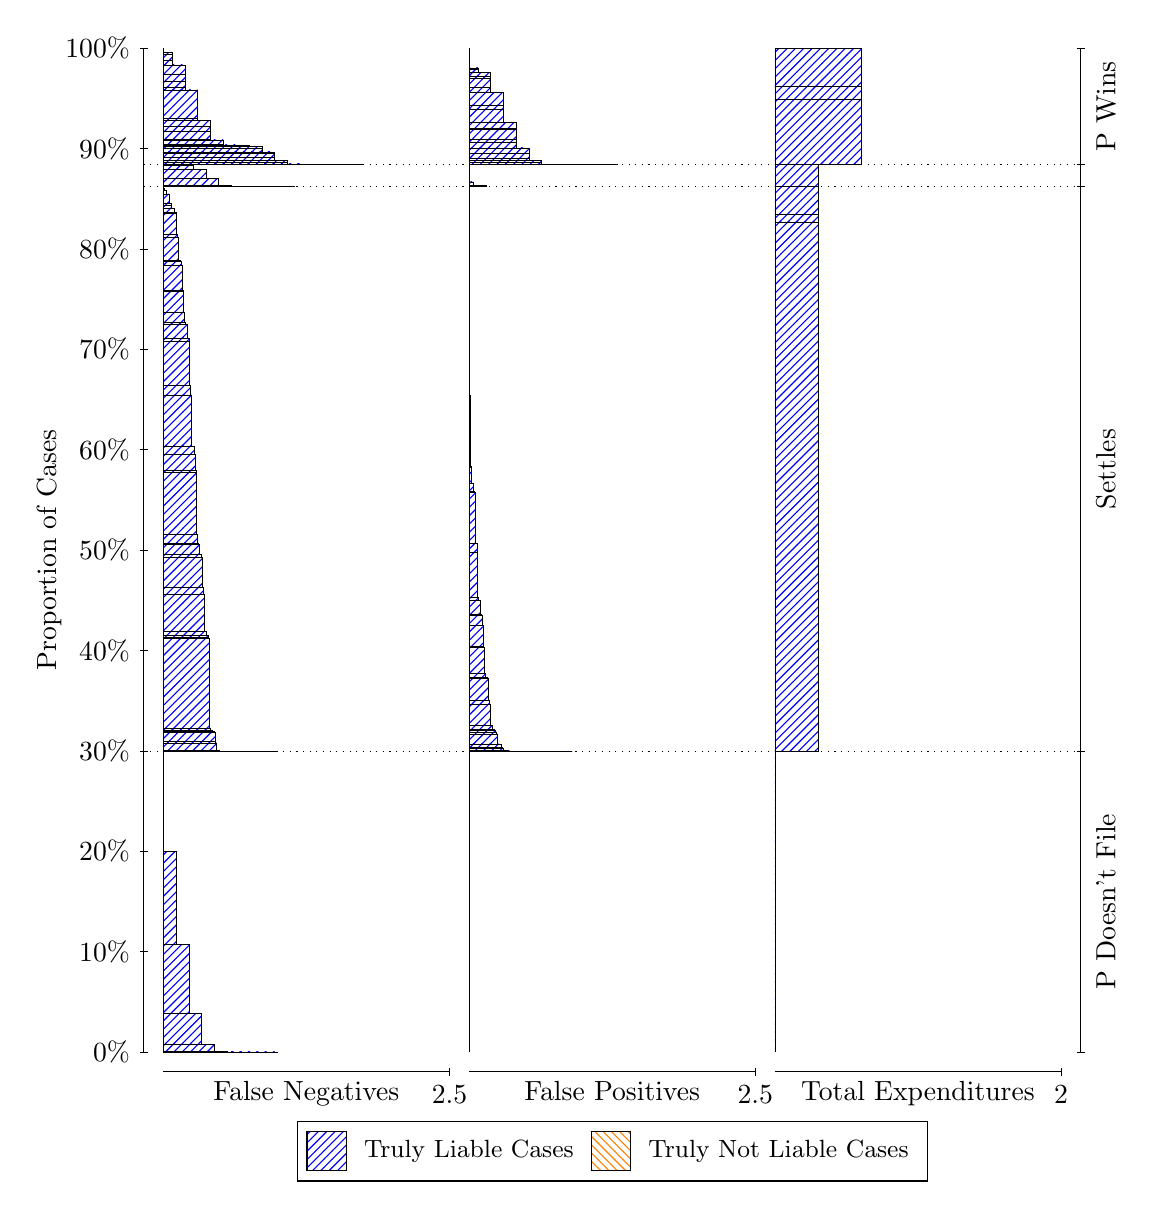
\begin{tikzpicture}
\draw[black, very thin] (1.5,1.75) -- (1.5,14.5);
\node[rotate=90, text=black, anchor=center] at (0.3, 8.125) {Proportion of Cases};
\draw[black, very thin] (1.45,1.75) -- (1.55,1.75);
\node[text=black, anchor=east] at (1.45, 1.75) {0\%};
\draw[black, very thin] (1.45,3.025) -- (1.55,3.025);
\node[text=black, anchor=east] at (1.45, 3.025) {10\%};
\draw[black, very thin] (1.45,4.3) -- (1.55,4.3);
\node[text=black, anchor=east] at (1.45, 4.3) {20\%};
\draw[black, very thin] (1.45,5.575) -- (1.55,5.575);
\node[text=black, anchor=east] at (1.45, 5.575) {30\%};
\draw[black, very thin] (1.45,6.85) -- (1.55,6.85);
\node[text=black, anchor=east] at (1.45, 6.85) {40\%};
\draw[black, very thin] (1.45,8.125) -- (1.55,8.125);
\node[text=black, anchor=east] at (1.45, 8.125) {50\%};
\draw[black, very thin] (1.45,9.4) -- (1.55,9.4);
\node[text=black, anchor=east] at (1.45, 9.4) {60\%};
\draw[black, very thin] (1.45,10.675) -- (1.55,10.675);
\node[text=black, anchor=east] at (1.45, 10.675) {70\%};
\draw[black, very thin] (1.45,11.95) -- (1.55,11.95);
\node[text=black, anchor=east] at (1.45, 11.95) {80\%};
\draw[black, very thin] (1.45,13.225) -- (1.55,13.225);
\node[text=black, anchor=east] at (1.45, 13.225) {90\%};
\draw[black, very thin] (1.45,14.5) -- (1.55,14.5);
\node[text=black, anchor=east] at (1.45, 14.5) {100\%};

\draw[black, very thin] (13.4,1.75) -- (13.4,14.5);
\draw[black, very thin] (13.35,1.75) -- (13.45,1.75);
\node[anchor=west] at (13.35, 1.75) {};
\draw[black, very thin] (13.35,5.563) -- (13.45,5.563);
\node[anchor=west] at (13.35, 5.563) {};
\draw[black, very thin] (13.35,12.743) -- (13.45,12.743);
\node[anchor=west] at (13.35, 12.743) {};
\draw[black, very thin] (13.35,13.018) -- (13.45,13.018);
\node[anchor=west] at (13.35, 13.018) {};
\draw[black, very thin] (13.35,14.5) -- (13.45,14.5);
\node[anchor=west] at (13.35, 14.5) {};

\draw[black, very thin, pattern color=blue, pattern=north east lines] (1.75,1.75) rectangle (3.2033,1.75);
\draw[black, very thin, pattern color=blue, pattern=north east lines] (1.75,1.75) rectangle (3.0419,1.75);
\draw[black, very thin, pattern color=blue, pattern=north east lines] (1.75,1.75) rectangle (2.8804,1.75);
\draw[black, very thin, pattern color=blue, pattern=north east lines] (1.75,1.75) rectangle (2.7189,1.7503);
\draw[black, very thin, pattern color=blue, pattern=north east lines] (1.75,1.7503) rectangle (2.5574,1.7582);
\draw[black, very thin, pattern color=blue, pattern=north east lines] (1.75,1.7582) rectangle (2.3959,1.8434);
\draw[black, very thin, pattern color=blue, pattern=north east lines] (1.75,1.8434) rectangle (2.2344,2.2366);
\draw[black, very thin, pattern color=blue, pattern=north east lines] (1.75,2.2366) rectangle (2.073,3.1157);
\draw[black, very thin, pattern color=blue, pattern=north east lines] (1.75,3.1157) rectangle (1.9115,4.2995);
\draw[black, very thin, pattern color=orange, pattern=north west lines] (1.75,4.2995) rectangle (1.75,4.2995);
\draw[black, very thin, pattern color=blue, pattern=north east lines] (1.75,4.2995) rectangle (1.75,5.563);
\draw[black, very thin, pattern color=blue, pattern=north east lines] (1.75,5.563) rectangle (3.2033,5.563);
\draw[black, very thin, pattern color=blue, pattern=north east lines] (1.75,5.563) rectangle (3.1307,5.563);
\draw[black, very thin, pattern color=blue, pattern=north east lines] (1.75,5.563) rectangle (3.058,5.563);
\draw[black, very thin, pattern color=blue, pattern=north east lines] (1.75,5.563) rectangle (3.0419,5.563);
\draw[black, very thin, pattern color=blue, pattern=north east lines] (1.75,5.563) rectangle (2.9853,5.563);
\draw[black, very thin, pattern color=blue, pattern=north east lines] (1.75,5.563) rectangle (2.9692,5.563);
\draw[black, very thin, pattern color=blue, pattern=north east lines] (1.75,5.563) rectangle (2.9127,5.563);
\draw[black, very thin, pattern color=blue, pattern=north east lines] (1.75,5.563) rectangle (2.8965,5.563);
\draw[black, very thin, pattern color=blue, pattern=north east lines] (1.75,5.563) rectangle (2.8804,5.563);
\draw[black, very thin, pattern color=blue, pattern=north east lines] (1.75,5.563) rectangle (2.84,5.563);
\draw[black, very thin, pattern color=blue, pattern=north east lines] (1.75,5.563) rectangle (2.8239,5.563);
\draw[black, very thin, pattern color=blue, pattern=north east lines] (1.75,5.563) rectangle (2.8077,5.563);
\draw[black, very thin, pattern color=blue, pattern=north east lines] (1.75,5.563) rectangle (2.7673,5.563);
\draw[black, very thin, pattern color=blue, pattern=north east lines] (1.75,5.563) rectangle (2.7512,5.5631);
\draw[black, very thin, pattern color=blue, pattern=north east lines] (1.75,5.5631) rectangle (2.735,5.5631);
\draw[black, very thin, pattern color=blue, pattern=north east lines] (1.75,5.5631) rectangle (2.7189,5.5631);
\draw[black, very thin, pattern color=blue, pattern=north east lines] (1.75,5.5631) rectangle (2.6947,5.5631);
\draw[black, very thin, pattern color=blue, pattern=north east lines] (1.75,5.5631) rectangle (2.6785,5.5631);
\draw[black, very thin, pattern color=blue, pattern=north east lines] (1.75,5.5631) rectangle (2.6624,5.5631);
\draw[black, very thin, pattern color=blue, pattern=north east lines] (1.75,5.5631) rectangle (2.6462,5.5631);
\draw[black, very thin, pattern color=blue, pattern=north east lines] (1.75,5.5631) rectangle (2.622,5.5634);
\draw[black, very thin, pattern color=blue, pattern=north east lines] (1.75,5.5634) rectangle (2.6059,5.5634);
\draw[black, very thin, pattern color=blue, pattern=north east lines] (1.75,5.5634) rectangle (2.5897,5.5679);
\draw[black, very thin, pattern color=blue, pattern=north east lines] (1.75,5.5679) rectangle (2.5736,5.5687);
\draw[black, very thin, pattern color=blue, pattern=north east lines] (1.75,5.5687) rectangle (2.5574,5.5688);
\draw[black, very thin, pattern color=blue, pattern=north east lines] (1.75,5.5688) rectangle (2.5332,5.5692);
\draw[black, very thin, pattern color=blue, pattern=north east lines] (1.75,5.5692) rectangle (2.517,5.5695);
\draw[black, very thin, pattern color=blue, pattern=north east lines] (1.75,5.5695) rectangle (2.5009,5.5705);
\draw[black, very thin, pattern color=blue, pattern=north east lines] (1.75,5.5705) rectangle (2.4847,5.5709);
\draw[black, very thin, pattern color=blue, pattern=north east lines] (1.75,5.5709) rectangle (2.4767,5.572);
\draw[black, very thin, pattern color=blue, pattern=north east lines] (1.75,5.572) rectangle (2.4605,5.5784);
\draw[black, very thin, pattern color=blue, pattern=north east lines] (1.75,5.5784) rectangle (2.4444,5.5785);
\draw[black, very thin, pattern color=blue, pattern=north east lines] (1.75,5.5785) rectangle (2.4282,5.6751);
\draw[black, very thin, pattern color=blue, pattern=north east lines] (1.75,5.6751) rectangle (2.4121,5.6914);
\draw[black, very thin, pattern color=blue, pattern=north east lines] (1.75,5.6914) rectangle (2.404,5.8132);
\draw[black, very thin, pattern color=blue, pattern=north east lines] (1.75,5.8132) rectangle (2.3959,5.8181);
\draw[black, very thin, pattern color=blue, pattern=north east lines] (1.75,5.8181) rectangle (2.3717,5.8354);
\draw[black, very thin, pattern color=blue, pattern=north east lines] (1.75,5.8354) rectangle (2.3556,5.8409);
\draw[black, very thin, pattern color=blue, pattern=north east lines] (1.75,5.8409) rectangle (2.3394,5.8632);
\draw[black, very thin, pattern color=blue, pattern=north east lines] (1.75,5.8632) rectangle (2.3313,7.0047);
\draw[black, very thin, pattern color=blue, pattern=north east lines] (1.75,7.0047) rectangle (2.3233,7.0118);
\draw[black, very thin, pattern color=blue, pattern=north east lines] (1.75,7.0118) rectangle (2.3152,7.0387);
\draw[black, very thin, pattern color=blue, pattern=north east lines] (1.75,7.0387) rectangle (2.299,7.0876);
\draw[black, very thin, pattern color=blue, pattern=north east lines] (1.75,7.0876) rectangle (2.2829,7.0896);
\draw[black, very thin, pattern color=blue, pattern=north east lines] (1.75,7.0896) rectangle (2.2667,7.5598);
\draw[black, very thin, pattern color=blue, pattern=north east lines] (1.75,7.5598) rectangle (2.2506,7.6462);
\draw[black, very thin, pattern color=blue, pattern=north east lines] (1.75,7.6462) rectangle (2.2425,8.0312);
\draw[black, very thin, pattern color=blue, pattern=north east lines] (1.75,8.0312) rectangle (2.2344,8.0649);
\draw[black, very thin, pattern color=blue, pattern=north east lines] (1.75,8.0649) rectangle (2.2102,8.1922);
\draw[black, very thin, pattern color=blue, pattern=north east lines] (1.75,8.1922) rectangle (2.1941,8.2141);
\draw[black, very thin, pattern color=blue, pattern=north east lines] (1.75,8.2141) rectangle (2.1779,8.3216);
\draw[black, very thin, pattern color=blue, pattern=north east lines] (1.75,8.3216) rectangle (2.1699,9.114);
\draw[black, very thin, pattern color=blue, pattern=north east lines] (1.75,9.114) rectangle (2.1618,9.1364);
\draw[black, very thin, pattern color=blue, pattern=north east lines] (1.75,9.1364) rectangle (2.1537,9.3349);
\draw[black, very thin, pattern color=blue, pattern=north east lines] (1.75,9.3349) rectangle (2.1376,9.4366);
\draw[black, very thin, pattern color=blue, pattern=north east lines] (1.75,9.4366) rectangle (2.1214,9.4463);
\draw[black, very thin, pattern color=blue, pattern=north east lines] (1.75,9.4463) rectangle (2.1053,10.095);
\draw[black, very thin, pattern color=blue, pattern=north east lines] (1.75,10.095) rectangle (2.0891,10.216);
\draw[black, very thin, pattern color=blue, pattern=north east lines] (1.75,10.216) rectangle (2.081,10.778);
\draw[black, very thin, pattern color=blue, pattern=north east lines] (1.75,10.778) rectangle (2.073,10.819);
\draw[black, very thin, pattern color=blue, pattern=north east lines] (1.75,10.819) rectangle (2.0487,10.997);
\draw[black, very thin, pattern color=blue, pattern=north east lines] (1.75,10.997) rectangle (2.0326,11.014);
\draw[black, very thin, pattern color=blue, pattern=north east lines] (1.75,11.014) rectangle (2.0164,11.139);
\draw[black, very thin, pattern color=blue, pattern=north east lines] (1.75,11.139) rectangle (2.0084,11.406);
\draw[black, very thin, pattern color=blue, pattern=north east lines] (1.75,11.406) rectangle (2.0003,11.42);
\draw[black, very thin, pattern color=blue, pattern=north east lines] (1.75,11.42) rectangle (1.9922,11.747);
\draw[black, very thin, pattern color=blue, pattern=north east lines] (1.75,11.747) rectangle (1.9761,11.796);
\draw[black, very thin, pattern color=blue, pattern=north east lines] (1.75,11.796) rectangle (1.9599,11.805);
\draw[black, very thin, pattern color=blue, pattern=north east lines] (1.75,11.805) rectangle (1.9438,12.095);
\draw[black, very thin, pattern color=blue, pattern=north east lines] (1.75,12.095) rectangle (1.9276,12.138);
\draw[black, very thin, pattern color=blue, pattern=north east lines] (1.75,12.138) rectangle (1.9196,12.402);
\draw[black, very thin, pattern color=blue, pattern=north east lines] (1.75,12.402) rectangle (1.9115,12.412);
\draw[black, very thin, pattern color=blue, pattern=north east lines] (1.75,12.412) rectangle (1.8873,12.462);
\draw[black, very thin, pattern color=blue, pattern=north east lines] (1.75,12.462) rectangle (1.8711,12.465);
\draw[black, very thin, pattern color=blue, pattern=north east lines] (1.75,12.465) rectangle (1.855,12.499);
\draw[black, very thin, pattern color=blue, pattern=north east lines] (1.75,12.499) rectangle (1.8469,12.525);
\draw[black, very thin, pattern color=blue, pattern=north east lines] (1.75,12.525) rectangle (1.8388,12.527);
\draw[black, very thin, pattern color=blue, pattern=north east lines] (1.75,12.527) rectangle (1.8307,12.642);
\draw[black, very thin, pattern color=blue, pattern=north east lines] (1.75,12.642) rectangle (1.8146,12.647);
\draw[black, very thin, pattern color=blue, pattern=north east lines] (1.75,12.647) rectangle (1.7984,12.648);
\draw[black, very thin, pattern color=blue, pattern=north east lines] (1.75,12.648) rectangle (1.7823,12.689);
\draw[black, very thin, pattern color=blue, pattern=north east lines] (1.75,12.689) rectangle (1.7661,12.693);
\draw[black, very thin, pattern color=blue, pattern=north east lines] (1.75,12.693) rectangle (1.7581,12.725);
\draw[black, very thin, pattern color=orange, pattern=north west lines] (1.75,12.725) rectangle (1.75,12.725);
\draw[black, very thin, pattern color=blue, pattern=north east lines] (1.75,12.725) rectangle (1.75,12.743);
\draw[black, very thin, pattern color=blue, pattern=north east lines] (1.75,12.743) rectangle (3.4213,12.743);
\draw[black, very thin, pattern color=blue, pattern=north east lines] (1.75,12.743) rectangle (3.2599,12.743);
\draw[black, very thin, pattern color=blue, pattern=north east lines] (1.75,12.743) rectangle (3.0984,12.743);
\draw[black, very thin, pattern color=blue, pattern=north east lines] (1.75,12.743) rectangle (2.9369,12.743);
\draw[black, very thin, pattern color=blue, pattern=north east lines] (1.75,12.743) rectangle (2.7754,12.743);
\draw[black, very thin, pattern color=blue, pattern=north east lines] (1.75,12.743) rectangle (2.6139,12.757);
\draw[black, very thin, pattern color=blue, pattern=north east lines] (1.75,12.757) rectangle (2.4524,12.841);
\draw[black, very thin, pattern color=blue, pattern=north east lines] (1.75,12.841) rectangle (2.291,12.962);
\draw[black, very thin, pattern color=blue, pattern=north east lines] (1.75,12.962) rectangle (2.1295,13.01);
\draw[black, very thin, pattern color=blue, pattern=north east lines] (1.75,13.01) rectangle (1.968,13.018);
\draw[black, very thin, pattern color=orange, pattern=north west lines] (1.75,13.018) rectangle (1.75,13.018);
\draw[black, very thin, pattern color=blue, pattern=north east lines] (1.75,13.018) rectangle (4.2933,13.018);
\draw[black, very thin, pattern color=blue, pattern=north east lines] (1.75,13.018) rectangle (4.1319,13.018);
\draw[black, very thin, pattern color=blue, pattern=north east lines] (1.75,13.018) rectangle (3.9704,13.018);
\draw[black, very thin, pattern color=blue, pattern=north east lines] (1.75,13.018) rectangle (3.8089,13.018);
\draw[black, very thin, pattern color=blue, pattern=north east lines] (1.75,13.018) rectangle (3.8089,13.018);
\draw[black, very thin, pattern color=blue, pattern=north east lines] (1.75,13.018) rectangle (3.6474,13.019);
\draw[black, very thin, pattern color=blue, pattern=north east lines] (1.75,13.019) rectangle (3.6474,13.019);
\draw[black, very thin, pattern color=blue, pattern=north east lines] (1.75,13.019) rectangle (3.4859,13.029);
\draw[black, very thin, pattern color=blue, pattern=north east lines] (1.75,13.029) rectangle (3.4779,13.029);
\draw[black, very thin, pattern color=blue, pattern=north east lines] (1.75,13.029) rectangle (3.3244,13.046);
\draw[black, very thin, pattern color=blue, pattern=north east lines] (1.75,13.046) rectangle (3.3244,13.077);
\draw[black, very thin, pattern color=blue, pattern=north east lines] (1.75,13.077) rectangle (3.3164,13.077);
\draw[black, very thin, pattern color=blue, pattern=north east lines] (1.75,13.077) rectangle (3.163,13.113);
\draw[black, very thin, pattern color=blue, pattern=north east lines] (1.75,13.113) rectangle (3.163,13.162);
\draw[black, very thin, pattern color=blue, pattern=north east lines] (1.75,13.162) rectangle (3.163,13.182);
\draw[black, very thin, pattern color=blue, pattern=north east lines] (1.75,13.182) rectangle (3.1549,13.182);
\draw[black, very thin, pattern color=blue, pattern=north east lines] (1.75,13.182) rectangle (3.1549,13.182);
\draw[black, very thin, pattern color=blue, pattern=north east lines] (1.75,13.182) rectangle (3.0015,13.229);
\draw[black, very thin, pattern color=blue, pattern=north east lines] (1.75,13.229) rectangle (3.0015,13.253);
\draw[black, very thin, pattern color=blue, pattern=north east lines] (1.75,13.253) rectangle (2.9934,13.253);
\draw[black, very thin, pattern color=blue, pattern=north east lines] (1.75,13.253) rectangle (2.9934,13.253);
\draw[black, very thin, pattern color=blue, pattern=north east lines] (1.75,13.253) rectangle (2.84,13.265);
\draw[black, very thin, pattern color=blue, pattern=north east lines] (1.75,13.265) rectangle (2.8319,13.266);
\draw[black, very thin, pattern color=blue, pattern=north east lines] (1.75,13.266) rectangle (2.6785,13.266);
\draw[black, very thin, pattern color=blue, pattern=north east lines] (1.75,13.266) rectangle (2.6704,13.27);
\draw[black, very thin, pattern color=blue, pattern=north east lines] (1.75,13.27) rectangle (2.517,13.27);
\draw[black, very thin, pattern color=blue, pattern=north east lines] (1.75,13.27) rectangle (2.517,13.27);
\draw[black, very thin, pattern color=blue, pattern=north east lines] (1.75,13.27) rectangle (2.509,13.273);
\draw[black, very thin, pattern color=blue, pattern=north east lines] (1.75,13.273) rectangle (2.509,13.332);
\draw[black, very thin, pattern color=blue, pattern=north east lines] (1.75,13.332) rectangle (2.3556,13.332);
\draw[black, very thin, pattern color=blue, pattern=north east lines] (1.75,13.332) rectangle (2.3556,13.332);
\draw[black, very thin, pattern color=blue, pattern=north east lines] (1.75,13.332) rectangle (2.3475,13.335);
\draw[black, very thin, pattern color=blue, pattern=north east lines] (1.75,13.335) rectangle (2.3475,13.446);
\draw[black, very thin, pattern color=blue, pattern=north east lines] (1.75,13.446) rectangle (2.3475,13.503);
\draw[black, very thin, pattern color=blue, pattern=north east lines] (1.75,13.503) rectangle (2.3475,13.581);
\draw[black, very thin, pattern color=blue, pattern=north east lines] (1.75,13.581) rectangle (2.1941,13.581);
\draw[black, very thin, pattern color=blue, pattern=north east lines] (1.75,13.581) rectangle (2.1941,13.581);
\draw[black, very thin, pattern color=blue, pattern=north east lines] (1.75,13.581) rectangle (2.186,13.605);
\draw[black, very thin, pattern color=blue, pattern=north east lines] (1.75,13.605) rectangle (2.186,13.967);
\draw[black, very thin, pattern color=blue, pattern=north east lines] (1.75,13.967) rectangle (2.0326,13.967);
\draw[black, very thin, pattern color=blue, pattern=north east lines] (1.75,13.967) rectangle (2.0245,14.006);
\draw[black, very thin, pattern color=blue, pattern=north east lines] (1.75,14.006) rectangle (2.0245,14.08);
\draw[black, very thin, pattern color=blue, pattern=north east lines] (1.75,14.08) rectangle (2.0245,14.168);
\draw[black, very thin, pattern color=blue, pattern=north east lines] (1.75,14.168) rectangle (2.0245,14.285);
\draw[black, very thin, pattern color=blue, pattern=north east lines] (1.75,14.285) rectangle (1.863,14.342);
\draw[black, very thin, pattern color=blue, pattern=north east lines] (1.75,14.342) rectangle (1.863,14.422);
\draw[black, very thin, pattern color=blue, pattern=north east lines] (1.75,14.422) rectangle (1.863,14.444);
\draw[black, very thin, pattern color=orange, pattern=north west lines] (1.75,14.444) rectangle (1.75,14.444);
\draw[black, very thin, pattern color=blue, pattern=north east lines] (1.75,14.444) rectangle (1.75,14.5);
\draw[black, very thin, pattern color=orange, pattern=north west lines] (5.6333,1.75) rectangle (5.6333,1.75);
\draw[black, very thin, pattern color=blue, pattern=north east lines] (5.6333,1.75) rectangle (5.6333,5.563);
\draw[black, very thin, pattern color=orange, pattern=north west lines] (5.6333,5.563) rectangle (6.9413,5.563);
\draw[black, very thin, pattern color=blue, pattern=north east lines] (5.6333,5.563) rectangle (6.9413,5.563);
\draw[black, very thin, pattern color=orange, pattern=north west lines] (5.6333,5.563) rectangle (6.8687,5.563);
\draw[black, very thin, pattern color=blue, pattern=north east lines] (5.6333,5.563) rectangle (6.8687,5.563);
\draw[black, very thin, pattern color=orange, pattern=north west lines] (5.6333,5.563) rectangle (6.796,5.563);
\draw[black, very thin, pattern color=blue, pattern=north east lines] (5.6333,5.563) rectangle (6.796,5.563);
\draw[black, very thin, pattern color=blue, pattern=north east lines] (5.6333,5.563) rectangle (6.7799,5.563);
\draw[black, very thin, pattern color=blue, pattern=north east lines] (5.6333,5.563) rectangle (6.7072,5.563);
\draw[black, very thin, pattern color=orange, pattern=north west lines] (5.6333,5.563) rectangle (6.6507,5.563);
\draw[black, very thin, pattern color=blue, pattern=north east lines] (5.6333,5.563) rectangle (6.6507,5.563);
\draw[black, very thin, pattern color=blue, pattern=north east lines] (5.6333,5.563) rectangle (6.6345,5.563);
\draw[black, very thin, pattern color=blue, pattern=north east lines] (5.6333,5.563) rectangle (6.6184,5.563);
\draw[black, very thin, pattern color=orange, pattern=north west lines] (5.6333,5.563) rectangle (6.578,5.563);
\draw[black, very thin, pattern color=blue, pattern=north east lines] (5.6333,5.563) rectangle (6.578,5.563);
\draw[black, very thin, pattern color=blue, pattern=north east lines] (5.6333,5.563) rectangle (6.5457,5.563);
\draw[black, very thin, pattern color=orange, pattern=north west lines] (5.6333,5.563) rectangle (6.5053,5.563);
\draw[black, very thin, pattern color=blue, pattern=north east lines] (5.6333,5.563) rectangle (6.5053,5.563);
\draw[black, very thin, pattern color=blue, pattern=north east lines] (5.6333,5.563) rectangle (6.4892,5.563);
\draw[black, very thin, pattern color=blue, pattern=north east lines] (5.6333,5.563) rectangle (6.473,5.563);
\draw[black, very thin, pattern color=blue, pattern=north east lines] (5.6333,5.563) rectangle (6.4569,5.563);
\draw[black, very thin, pattern color=orange, pattern=north west lines] (5.6333,5.563) rectangle (6.4327,5.563);
\draw[black, very thin, pattern color=blue, pattern=north east lines] (5.6333,5.563) rectangle (6.4327,5.563);
\draw[black, very thin, pattern color=blue, pattern=north east lines] (5.6333,5.563) rectangle (6.4165,5.563);
\draw[black, very thin, pattern color=blue, pattern=north east lines] (5.6333,5.563) rectangle (6.3842,5.563);
\draw[black, very thin, pattern color=orange, pattern=north west lines] (5.6333,5.563) rectangle (6.36,5.563);
\draw[black, very thin, pattern color=blue, pattern=north east lines] (5.6333,5.563) rectangle (6.36,5.563);
\draw[black, very thin, pattern color=blue, pattern=north east lines] (5.6333,5.563) rectangle (6.3439,5.563);
\draw[black, very thin, pattern color=blue, pattern=north east lines] (5.6333,5.563) rectangle (6.3277,5.563);
\draw[black, very thin, pattern color=blue, pattern=north east lines] (5.6333,5.563) rectangle (6.3116,5.5632);
\draw[black, very thin, pattern color=blue, pattern=north east lines] (5.6333,5.5632) rectangle (6.2954,5.5632);
\draw[black, very thin, pattern color=orange, pattern=north west lines] (5.6333,5.5632) rectangle (6.2873,5.5632);
\draw[black, very thin, pattern color=blue, pattern=north east lines] (5.6333,5.5632) rectangle (6.2873,5.5632);
\draw[black, very thin, pattern color=blue, pattern=north east lines] (5.6333,5.5632) rectangle (6.2712,5.5632);
\draw[black, very thin, pattern color=blue, pattern=north east lines] (5.6333,5.5632) rectangle (6.255,5.5632);
\draw[black, very thin, pattern color=blue, pattern=north east lines] (5.6333,5.5632) rectangle (6.2227,5.5641);
\draw[black, very thin, pattern color=orange, pattern=north west lines] (5.6333,5.5641) rectangle (6.2147,5.5641);
\draw[black, very thin, pattern color=blue, pattern=north east lines] (5.6333,5.5641) rectangle (6.2147,5.5643);
\draw[black, very thin, pattern color=blue, pattern=north east lines] (5.6333,5.5643) rectangle (6.1985,5.5659);
\draw[black, very thin, pattern color=blue, pattern=north east lines] (5.6333,5.5659) rectangle (6.1824,5.5659);
\draw[black, very thin, pattern color=blue, pattern=north east lines] (5.6333,5.5659) rectangle (6.1662,5.566);
\draw[black, very thin, pattern color=blue, pattern=north east lines] (5.6333,5.566) rectangle (6.1501,5.5747);
\draw[black, very thin, pattern color=orange, pattern=north west lines] (5.6333,5.5747) rectangle (6.142,5.5747);
\draw[black, very thin, pattern color=blue, pattern=north east lines] (5.6333,5.5747) rectangle (6.142,5.5747);
\draw[black, very thin, pattern color=blue, pattern=north east lines] (5.6333,5.5747) rectangle (6.1339,5.5753);
\draw[black, very thin, pattern color=blue, pattern=north east lines] (5.6333,5.5753) rectangle (6.1259,5.5773);
\draw[black, very thin, pattern color=blue, pattern=north east lines] (5.6333,5.5773) rectangle (6.1097,5.5773);
\draw[black, very thin, pattern color=blue, pattern=north east lines] (5.6333,5.5773) rectangle (6.0936,5.5803);
\draw[black, very thin, pattern color=orange, pattern=north west lines] (5.6333,5.5803) rectangle (6.0693,5.5803);
\draw[black, very thin, pattern color=blue, pattern=north east lines] (5.6333,5.5803) rectangle (6.0693,5.5812);
\draw[black, very thin, pattern color=blue, pattern=north east lines] (5.6333,5.5812) rectangle (6.0613,5.613);
\draw[black, very thin, pattern color=blue, pattern=north east lines] (5.6333,5.613) rectangle (6.0532,5.617);
\draw[black, very thin, pattern color=blue, pattern=north east lines] (5.6333,5.617) rectangle (6.037,5.6574);
\draw[black, very thin, pattern color=blue, pattern=north east lines] (5.6333,5.6574) rectangle (6.0209,5.6587);
\draw[black, very thin, pattern color=blue, pattern=north east lines] (5.6333,5.6587) rectangle (6.0047,5.6638);
\draw[black, very thin, pattern color=blue, pattern=north east lines] (5.6333,5.6638) rectangle (5.9886,5.7791);
\draw[black, very thin, pattern color=blue, pattern=north east lines] (5.6333,5.7791) rectangle (5.9805,5.7809);
\draw[black, very thin, pattern color=blue, pattern=north east lines] (5.6333,5.7809) rectangle (5.9724,5.8071);
\draw[black, very thin, pattern color=blue, pattern=north east lines] (5.6333,5.8071) rectangle (5.9644,5.8407);
\draw[black, very thin, pattern color=blue, pattern=north east lines] (5.6333,5.8407) rectangle (5.9482,5.8434);
\draw[black, very thin, pattern color=blue, pattern=north east lines] (5.6333,5.8434) rectangle (5.9321,5.8936);
\draw[black, very thin, pattern color=blue, pattern=north east lines] (5.6333,5.8936) rectangle (5.9079,5.9041);
\draw[black, very thin, pattern color=blue, pattern=north east lines] (5.6333,5.9041) rectangle (5.8998,6.1676);
\draw[black, very thin, pattern color=blue, pattern=north east lines] (5.6333,6.1676) rectangle (5.8917,6.2109);
\draw[black, very thin, pattern color=blue, pattern=north east lines] (5.6333,6.2109) rectangle (5.8756,6.5012);
\draw[black, very thin, pattern color=blue, pattern=north east lines] (5.6333,6.5012) rectangle (5.8594,6.5099);
\draw[black, very thin, pattern color=blue, pattern=north east lines] (5.6333,6.5099) rectangle (5.8433,6.5583);
\draw[black, very thin, pattern color=blue, pattern=north east lines] (5.6333,6.5583) rectangle (5.8271,6.8855);
\draw[black, very thin, pattern color=blue, pattern=north east lines] (5.6333,6.8855) rectangle (5.819,6.8993);
\draw[black, very thin, pattern color=blue, pattern=north east lines] (5.6333,6.8993) rectangle (5.811,7.1668);
\draw[black, very thin, pattern color=blue, pattern=north east lines] (5.6333,7.1668) rectangle (5.8029,7.2918);
\draw[black, very thin, pattern color=blue, pattern=north east lines] (5.6333,7.2918) rectangle (5.7867,7.3091);
\draw[black, very thin, pattern color=blue, pattern=north east lines] (5.6333,7.3091) rectangle (5.7706,7.4864);
\draw[black, very thin, pattern color=blue, pattern=north east lines] (5.6333,7.4864) rectangle (5.7464,7.5275);
\draw[black, very thin, pattern color=blue, pattern=north east lines] (5.6333,7.5275) rectangle (5.7383,8.0901);
\draw[black, very thin, pattern color=blue, pattern=north east lines] (5.6333,8.0901) rectangle (5.7302,8.2111);
\draw[black, very thin, pattern color=blue, pattern=north east lines] (5.6333,8.2111) rectangle (5.7141,8.8595);
\draw[black, very thin, pattern color=blue, pattern=north east lines] (5.6333,8.8595) rectangle (5.6979,8.8692);
\draw[black, very thin, pattern color=blue, pattern=north east lines] (5.6333,8.8692) rectangle (5.6818,8.9709);
\draw[black, very thin, pattern color=blue, pattern=north east lines] (5.6333,8.9709) rectangle (5.6656,9.1693);
\draw[black, very thin, pattern color=blue, pattern=north east lines] (5.6333,9.1693) rectangle (5.6576,9.1918);
\draw[black, very thin, pattern color=blue, pattern=north east lines] (5.6333,9.1918) rectangle (5.6495,9.9841);
\draw[black, very thin, pattern color=blue, pattern=north east lines] (5.6333,9.9841) rectangle (5.6414,10.092);
\draw[black, very thin, pattern color=blue, pattern=north east lines] (5.6333,10.092) rectangle (5.6333,12.743);
\draw[black, very thin, pattern color=orange, pattern=north west lines] (5.6333,12.743) rectangle (5.8513,12.743);
\draw[black, very thin, pattern color=blue, pattern=north east lines] (5.6333,12.743) rectangle (5.8513,12.751);
\draw[black, very thin, pattern color=blue, pattern=north east lines] (5.6333,12.751) rectangle (5.6899,12.799);
\draw[black, very thin, pattern color=blue, pattern=north east lines] (5.6333,12.799) rectangle (5.6333,13.018);
\draw[black, very thin, pattern color=orange, pattern=north west lines] (5.6333,13.018) rectangle (7.5227,13.018);
\draw[black, very thin, pattern color=blue, pattern=north east lines] (5.6333,13.018) rectangle (7.5227,13.018);
\draw[black, very thin, pattern color=orange, pattern=north west lines] (5.6333,13.018) rectangle (7.3612,13.018);
\draw[black, very thin, pattern color=blue, pattern=north east lines] (5.6333,13.018) rectangle (7.3612,13.018);
\draw[black, very thin, pattern color=blue, pattern=north east lines] (5.6333,13.018) rectangle (7.1997,13.018);
\draw[black, very thin, pattern color=orange, pattern=north west lines] (5.6333,13.018) rectangle (7.1997,13.018);
\draw[black, very thin, pattern color=blue, pattern=north east lines] (5.6333,13.018) rectangle (7.1997,13.018);
\draw[black, very thin, pattern color=blue, pattern=north east lines] (5.6333,13.018) rectangle (7.0382,13.018);
\draw[black, very thin, pattern color=blue, pattern=north east lines] (5.6333,13.018) rectangle (7.0382,13.018);
\draw[black, very thin, pattern color=orange, pattern=north west lines] (5.6333,13.018) rectangle (7.0382,13.018);
\draw[black, very thin, pattern color=blue, pattern=north east lines] (5.6333,13.018) rectangle (7.0382,13.018);
\draw[black, very thin, pattern color=orange, pattern=north west lines] (5.6333,13.018) rectangle (6.8767,13.018);
\draw[black, very thin, pattern color=blue, pattern=north east lines] (5.6333,13.018) rectangle (6.8767,13.018);
\draw[black, very thin, pattern color=blue, pattern=north east lines] (5.6333,13.018) rectangle (6.8767,13.019);
\draw[black, very thin, pattern color=blue, pattern=north east lines] (5.6333,13.019) rectangle (6.8767,13.019);
\draw[black, very thin, pattern color=orange, pattern=north west lines] (5.6333,13.019) rectangle (6.7153,13.019);
\draw[black, very thin, pattern color=blue, pattern=north east lines] (5.6333,13.019) rectangle (6.7153,13.025);
\draw[black, very thin, pattern color=blue, pattern=north east lines] (5.6333,13.025) rectangle (6.7153,13.026);
\draw[black, very thin, pattern color=blue, pattern=north east lines] (5.6333,13.026) rectangle (6.5538,13.043);
\draw[black, very thin, pattern color=orange, pattern=north west lines] (5.6333,13.043) rectangle (6.5538,13.043);
\draw[black, very thin, pattern color=blue, pattern=north east lines] (5.6333,13.043) rectangle (6.5538,13.074);
\draw[black, very thin, pattern color=blue, pattern=north east lines] (5.6333,13.074) rectangle (6.3923,13.096);
\draw[black, very thin, pattern color=blue, pattern=north east lines] (5.6333,13.096) rectangle (6.3923,13.165);
\draw[black, very thin, pattern color=orange, pattern=north west lines] (5.6333,13.165) rectangle (6.3923,13.165);
\draw[black, very thin, pattern color=blue, pattern=north east lines] (5.6333,13.165) rectangle (6.3923,13.233);
\draw[black, very thin, pattern color=blue, pattern=north east lines] (5.6333,13.233) rectangle (6.2308,13.297);
\draw[black, very thin, pattern color=blue, pattern=north east lines] (5.6333,13.297) rectangle (6.2308,13.34);
\draw[black, very thin, pattern color=orange, pattern=north west lines] (5.6333,13.34) rectangle (6.2308,13.34);
\draw[black, very thin, pattern color=blue, pattern=north east lines] (5.6333,13.34) rectangle (6.2308,13.471);
\draw[black, very thin, pattern color=blue, pattern=north east lines] (5.6333,13.471) rectangle (6.2308,13.476);
\draw[black, very thin, pattern color=blue, pattern=north east lines] (5.6333,13.476) rectangle (6.2308,13.551);
\draw[black, very thin, pattern color=orange, pattern=north west lines] (5.6333,13.551) rectangle (6.2227,13.551);
\draw[black, very thin, pattern color=blue, pattern=north east lines] (5.6333,13.551) rectangle (6.2227,13.551);
\draw[black, very thin, pattern color=blue, pattern=north east lines] (5.6333,13.551) rectangle (6.0693,13.726);
\draw[black, very thin, pattern color=blue, pattern=north east lines] (5.6333,13.726) rectangle (6.0693,13.778);
\draw[black, very thin, pattern color=blue, pattern=north east lines] (5.6333,13.778) rectangle (6.0693,13.937);
\draw[black, very thin, pattern color=blue, pattern=north east lines] (5.6333,13.937) rectangle (6.0613,13.937);
\draw[black, very thin, pattern color=orange, pattern=north west lines] (5.6333,13.937) rectangle (6.0613,13.937);
\draw[black, very thin, pattern color=blue, pattern=north east lines] (5.6333,13.937) rectangle (6.0613,13.937);
\draw[black, very thin, pattern color=blue, pattern=north east lines] (5.6333,13.937) rectangle (5.9079,13.998);
\draw[black, very thin, pattern color=blue, pattern=north east lines] (5.6333,13.998) rectangle (5.9079,14.12);
\draw[black, very thin, pattern color=blue, pattern=north east lines] (5.6333,14.12) rectangle (5.9079,14.147);
\draw[black, very thin, pattern color=blue, pattern=north east lines] (5.6333,14.147) rectangle (5.9079,14.186);
\draw[black, very thin, pattern color=blue, pattern=north east lines] (5.6333,14.186) rectangle (5.8998,14.186);
\draw[black, very thin, pattern color=orange, pattern=north west lines] (5.6333,14.186) rectangle (5.8998,14.186);
\draw[black, very thin, pattern color=blue, pattern=north east lines] (5.6333,14.186) rectangle (5.8998,14.186);
\draw[black, very thin, pattern color=blue, pattern=north east lines] (5.6333,14.186) rectangle (5.7464,14.227);
\draw[black, very thin, pattern color=blue, pattern=north east lines] (5.6333,14.227) rectangle (5.7464,14.229);
\draw[black, very thin, pattern color=blue, pattern=north east lines] (5.6333,14.229) rectangle (5.7464,14.247);
\draw[black, very thin, pattern color=blue, pattern=north east lines] (5.6333,14.247) rectangle (5.7383,14.247);
\draw[black, very thin, pattern color=orange, pattern=north west lines] (5.6333,14.247) rectangle (5.7383,14.247);
\draw[black, very thin, pattern color=blue, pattern=north east lines] (5.6333,14.247) rectangle (5.7383,14.247);
\draw[black, very thin, pattern color=orange, pattern=north west lines] (5.6333,14.247) rectangle (5.6333,14.247);
\draw[black, very thin, pattern color=blue, pattern=north east lines] (5.6333,14.247) rectangle (5.6333,14.5);
\draw[black, very thin, pattern color=orange, pattern=north west lines] (9.5167,1.75) rectangle (9.5167,1.75);
\draw[black, very thin, pattern color=blue, pattern=north east lines] (9.5167,1.75) rectangle (9.5167,5.563);
\draw[black, very thin, pattern color=orange, pattern=north west lines] (9.5167,5.563) rectangle (10.062,5.563);
\draw[black, very thin, pattern color=blue, pattern=north east lines] (9.5167,5.563) rectangle (10.062,12.292);
\draw[black, very thin, pattern color=orange, pattern=north west lines] (9.5167,12.292) rectangle (10.062,12.292);
\draw[black, very thin, pattern color=blue, pattern=north east lines] (9.5167,12.292) rectangle (10.062,12.384);
\draw[black, very thin, pattern color=orange, pattern=north west lines] (9.5167,12.384) rectangle (10.062,12.384);
\draw[black, very thin, pattern color=blue, pattern=north east lines] (9.5167,12.384) rectangle (10.062,12.743);
\draw[black, very thin, pattern color=orange, pattern=north west lines] (9.5167,12.743) rectangle (10.062,12.743);
\draw[black, very thin, pattern color=blue, pattern=north east lines] (9.5167,12.743) rectangle (10.062,13.018);
\draw[black, very thin, pattern color=orange, pattern=north west lines] (9.5167,13.018) rectangle (10.607,13.018);
\draw[black, very thin, pattern color=blue, pattern=north east lines] (9.5167,13.018) rectangle (10.607,13.843);
\draw[black, very thin, pattern color=orange, pattern=north west lines] (9.5167,13.843) rectangle (10.607,13.843);
\draw[black, very thin, pattern color=blue, pattern=north east lines] (9.5167,13.843) rectangle (10.607,14.01);
\draw[black, very thin, pattern color=orange, pattern=north west lines] (9.5167,14.01) rectangle (10.607,14.01);
\draw[black, very thin, pattern color=blue, pattern=north east lines] (9.5167,14.01) rectangle (10.607,14.5);
\draw[black, dotted] (1.5,5.563) -- (13.4,5.563);
\draw[black, dotted] (1.5,12.743) -- (13.4,12.743);
\draw[black, dotted] (1.5,13.018) -- (13.4,13.018);
\draw[black, very thin] (1.75,1.5) -- (5.3833,1.5);
\node[text=black, anchor=north] at (3.5667, 1.5) {False Negatives};
\draw[black, very thin] (5.3833,1.45) -- (5.3833,1.55);
\node[text=black, anchor=north] at (5.3833, 1.45) {2.5};

\draw[black, very thin] (5.6333,1.5) -- (9.2667,1.5);
\node[text=black, anchor=north] at (7.45, 1.5) {False Positives};
\draw[black, very thin] (9.2667,1.45) -- (9.2667,1.55);
\node[text=black, anchor=north] at (9.2667, 1.45) {2.5};

\draw[black, very thin] (9.5167,1.5) -- (13.15,1.5);
\node[text=black, anchor=north] at (11.333, 1.5) {Total Expenditures};
\draw[black, very thin] (13.15,1.45) -- (13.15,1.55);
\node[text=black, anchor=north] at (13.15, 1.45) {2};

\node[text=black, centered, rotate=90] at (13.72, 3.6565) {P Doesn't File};
\node[text=black, centered, rotate=90] at (13.72, 9.1529) {Settles};

\node[text=black, centered, rotate=90] at (13.72, 13.759) {P Wins};

\draw (7.449999999999999,1.5) node[draw=none] (baseCoordinate) {};
\begin{scope}[align=center]
        \matrix[scale=0.5, draw=black, below=0.5cm of baseCoordinate, nodes={draw}, column sep=0.1cm]{
            \node[rectangle, draw, minimum width=0.5cm, minimum height=0.5cm, pattern color=blue, pattern=north east lines] {}; &
            \node[draw=none, font=\small, text=black] (B) {Truly Liable Cases}; &
            \node[rectangle, draw, minimum width=0.5cm, minimum height=0.5cm, pattern color=orange, pattern=north west lines] {}; &
            \node[draw=none, font=\small, text=black] (B) {Truly Not Liable Cases}; \\
            };
\end{scope}

\end{tikzpicture}
\end{document}